\section{Research Questions}
Our research questions aim to discover how people perceive and discuss armed conflicts. We suspect some of the same biases that affect traditional media will also affect social media. This may be especially true for Reddit due to its news-driven process. Nonetheless, it is unlikely that such different sources would produce exactly the same phenomena. 

Our data set consists of approximately 426GB of Reddit data, ranging from the year 2012 to the year 2014. We cross-referenced this with data from the Armed Conflicts Database, collecting a list of 48 conflicts that are considered by the Database to have been active in at least one of those years. The status is determined by experts working for the Database who are monitoring trends of armed conflicts worldwide. We used active conflicts to ensure none were seen by commenters as purely historical. See Figure~\ref{conflicts} for a summary of where the conflicts occurred. 

We gathered Reddit comments that are relevant to each of the 48 conflicts by searching for comments in every single subreddit. We compiled sets of keywords for every conflict then collected comments which matched them. For instance, if a comment contained the phrase ``Syrian Civil War'', we would mark that comment as relevant to the conflict in Syria. Most of our keywords were fairly specific; nonetheless, we sought to counter false positives by having a sufficiently large data set. The biggest source of comments was the ``worldnews'' subreddit, with many of the others coming from similar subreddits.

\begin{figure}
\centering
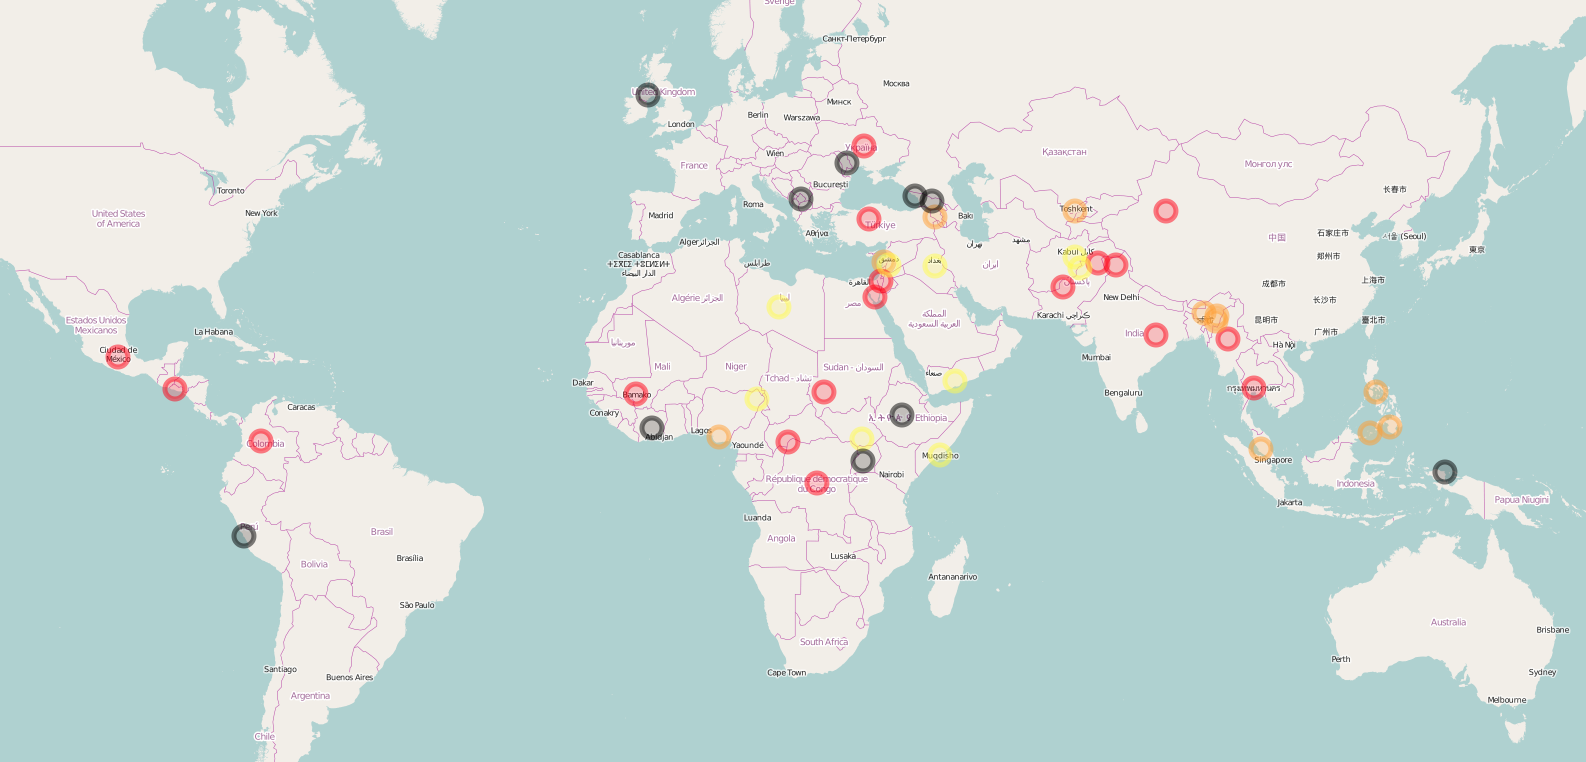
\includegraphics[width=0.9\columnwidth]{map}
\caption{A map of the 48 conflicts. Black, yellow, orange and red circles indicate the current level of intensity as rated by the Armed Conflict Database: archived, low, medium and high, respectively.}
\label{conflicts}
\end{figure}